\documentclass[12pt,executivepaper]{article}
\usepackage[utf8]{inputenc}
\usepackage[spanish]{babel}
\usepackage{amsmath}
\usepackage{amsfonts}
\usepackage{amssymb}
\usepackage{graphics}
\usepackage{graphicx}
\usepackage[left=1cm,right=1cm,top=2cm,bottom=2cm]{geometry}
\usepackage{imakeidx}
\makeindex[columns=3, title=Alphabetical Index, intoc]
\usepackage{listings}
\usepackage{xcolor}
\usepackage{multicol}
\usepackage{changepage}
\usepackage{float}
\usepackage{cite}
\usepackage{url}
\usepackage{hyperref}
\usepackage{pdfpages}

\definecolor{codegreen}{rgb}{0,0.6,0}
\definecolor{codegray}{rgb}{0.5,0.5,0.5}
\definecolor{codepurple}{rgb}{0.58,0,0.82}
\definecolor{backcolour}{rgb}{0.95,0.95,0.92}

\lstdefinestyle{mystyle}{
    backgroundcolor=\color{backcolour},
    commentstyle=\color{codegreen},
    keywordstyle=\color{magenta},
    numberstyle=\tiny\color{codegray},
    stringstyle=\color{codepurple},
    basicstyle=\ttfamily\footnotesize,
    breakatwhitespace=false,
    breaklines=true,
    captionpos=b,
    keepspaces=true,
    numbers=left,
    numbersep=5pt,
    showspaces=false,
    showstringspaces=false,
    showtabs=false,
    tabsize=3
}

\lstset{style=mystyle}
\author{González Pardo Adrian}
\date{Marzo 2020}

\title{Reporte de practica 5}
\newcommand\tab[1][1cm]{\hspace*{#1}}
\begin{document}
\maketitle
\section{Código C++}
\begin{center}
    \lstinputlisting[language=c++]{./sources/registros.cpp}
    \textit{Código fuente de archivo de registros}\\
\end{center}
\clearpage
\section{Captura de simulaciones}
\begin{center}
    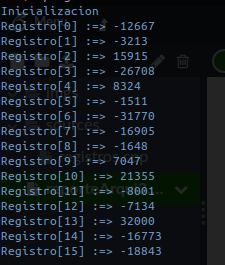
\includegraphics[scale=1]{imgs/uno.png}\\
    \textit{Figura 0: Inicialización del programa con números random}\\
    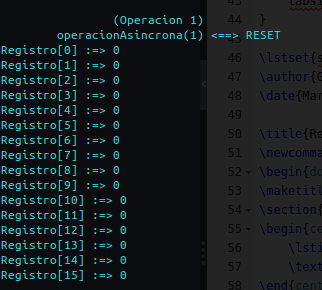
\includegraphics[scale=1]{imgs/dos.png}\\
    \textit{Figura 1: Operación 1 "Reset"}\\
    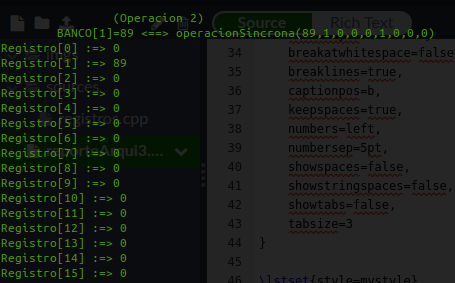
\includegraphics[scale=1]{imgs/tres.png}\\
    \textit{Figura 2: Operación 2 "Banco[1]=89"}\\
    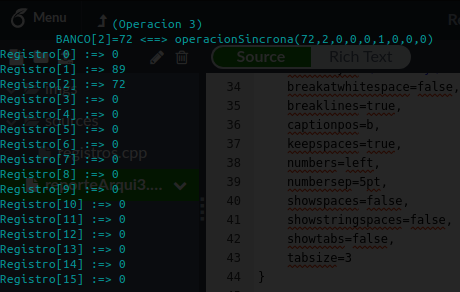
\includegraphics[scale=1]{imgs/cuatro.png}\\
    \textit{Figura 3: Operación 3 "Banco[2]=72"}\\
    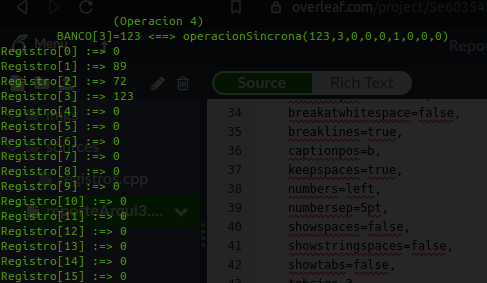
\includegraphics[scale=0.9]{imgs/cinco.png}\\
    \textit{Figura 4: Operación 4 "Banco[3]=123"}\\
    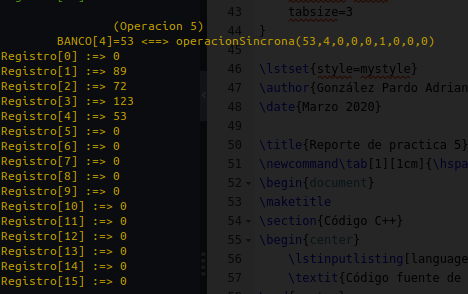
\includegraphics[scale=0.9]{imgs/seis.png}\\
    \textit{Figura 5: Operación 5 "Banco[4]=53"}\\
    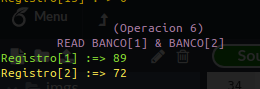
\includegraphics[scale=1]{imgs/siete.png}\\
    \textit{Figura 6: Operación 6 "READ Banco[1] \& Banco[2]"}\\
    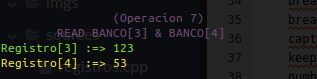
\includegraphics[scale=1]{imgs/ocho.png}\\
    \textit{Figura 7: Operación 7 "READ Banco[3] \& Banco[4]"}\\
    
    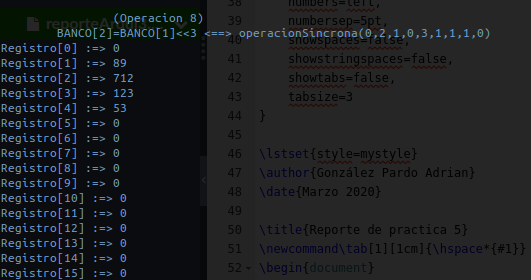
\includegraphics[scale=0.85]{imgs/nueve.png}\\
    \textit{Figura 8: Operación 8 "Banco[2]=Banco[1]$<<$3"}\\
    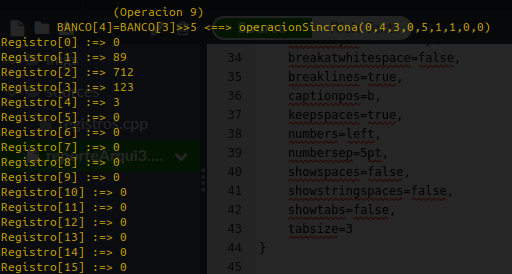
\includegraphics[scale=0.9]{imgs/diez.png}\\
    \textit{Figura 9: Operación 9 "Banco[4]=Banco[3]$>>$5"}\\
    
    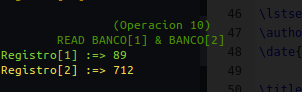
\includegraphics[scale=1]{imgs/once.png}\\
    \textit{Figura 10: Operación 10 "READ Banco[1] \& Banco[2]"}\\
    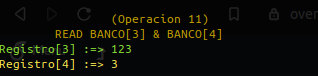
\includegraphics[scale=1]{imgs/doce.png}\\
    \textit{Figura 11: Operación 11 "READ Banco[3] \& Banco[4]"}\\
    
    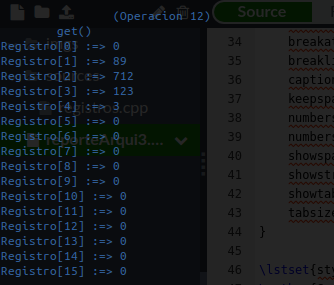
\includegraphics[scale=1]{imgs/trece.png}\\
    \textit{Figura 12: Operación 12 "GET()"}\\
    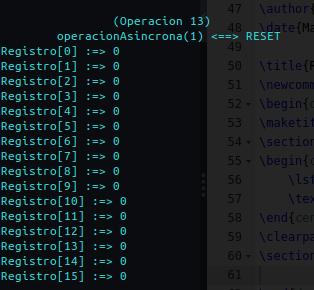
\includegraphics[scale=1]{imgs/catorce.png}\\
    \textit{Figura 13: Operación 13 "Reset"}\\
    
\end{center}
\end{document}